\chapter{Conclusion}
In this paper the problem of registration of 3D scans was studied from three points of view. First, a survey of previously developed point cloud registration algorithms was presented, especially variants of \gls{icp}. Some techniques as well as the mathematical theory behind it were laid out in more detail. 

Secondly, the stability of standard \gls{icp} registration was tested experimentally with regard to different resolution point clouds, and different camera view points. For this \gls{icp} registrations were run on a large number of different point clouds and results were collected and analyzed.

Thirdly, an attempt was made to develop an error metric specifically for the case where the point clouds have different resolutions. For artificially generated point clouds, positive results were obtained, but the error metric could not be applied to real scans.


\section{Discussion}
The goal of improving improving fine registration of point clouds with different resolutions could not be reached, but it could be shown that an approach based on the comparison of probability distributions originating from the point dispersion patterns, is possible. Some interesting results were obtained, which suggest that the described method could be further developed.

The method takes the dispersion of points on surfaces into account as additional information about the surface geometry. Moreover, it is not based on the assumption that closest point correspondences are a sufficient approximation to true correspondences. Error metrics based on point correspondences, like standard point-to-point \gls{icp}, assume that with the optimal alignment corresponding points will coincide on average, and that remaining errors due to different resolutions and dispersions, will even out. The experiments in chapter \ref{ch:experiments} have shown that this is no longer accurate when resolution differences are strong.

This error metric compares the \gls{acdh} to what it should be like when surfaces are perfectly aligned. The surface of $P$ could also be reconstructed by putting mesh triangles on neighboring points from the range image's image space. This would not need analysis of the lattice that the projected points form on the surfaces. However the shape of the surface joining the neighboring points is unknown, and any surface reconstruction means that one possible interpolation of it gets favored. Comparing sample points $q$ to that surface means that the error of this assumption gets propagated.

With the idea presented here this is not the case. Instead the metric would reach its minimum only in the hypothetical case where the surface is perfectly planar and the samples are perfectly dense and evenly distributed.


\section{Possible developments}
The problem of minimizing $e_{\chi}$ could be addressed by randomly sampling the neighboring transformations space at each iteration if \gls{icp}. Alternately, it might be possible to set the weights of the correspondences to values that would ``pull'' the \gls{roi} histogram into the intended shape.

The premise was that information about the true error $e(\matr{M'})$ is ``encoded'' within the coarsely aligned point clouds $P$ and $Q$, and can be extracted by analyzing their point dispersion patterns, or other attributes. Based on this it may be possible to find apply \emph{data mining} or similar artificial intelligence techniques on the problem. By using a large testing set, automatically find a function $f$ that best fits $f(P, Q, \matr{M'}, x_1, x_2, \cdots, x_m) \approx e(\matr{M'})$, where $x_i$ are various features extracted from $P$ and $Q$. These would for instance include metrics of the closest point distance histograms.

In general, it seems that the patterns that the dispersions of range image points produce on object surfaces, have not been formally studied in literature about point clouds registration. During the review of literature, no articles have been found which relate the arrangement of range image points to mathematical theory on parallelogram lattices.

When working on one single range image point cloud, it can be sufficient to look at the pixels in image space. However when two range images with different projection parameters become involved, this is no longer the case. Because the exact camera parameters for back-projecting three-dimensional coordinates onto the image space are unknown, the only ``view'' one gets from \emph{another} camera's image space is the pattern that its points form on object surfaces.

Obviously there is some regularity in the point dispersion pattern. So it is possible to predict, by looking at the pattern, where points \emph{should} lie based on hypothesis about the object surface and camera. Comparing this to where those points actually lie then allows to refute or reinforce those hypothesis.

Probabilistic techniques such as Generalized ICP, \gls{ndt} or approaches solely based on (estimated) normal vectors, all ``blur'' away the point dispersion and reduce it to a smooth distribution with some level of uncertainty.


\section{Practice}
However, in practice, high- to low-resolution registration problems can usually already be solved using one of the variants of \gls{icp} or another fine registration algorithm. It has been shown in section \ref{sec:icp_reg_exp} that \gls{icp} is relatively insensitive to resolution differences.

In this figure \ref{fig:ddp_good} the high and low resolution versions of the dessus-de-porte were registered with a standard point-to-point \gls{icp}. The only additional constraint was that only $20000$ random points were chosen for each iteration, and points located too far away from the centroid were ignored.

\begin{figure}[h]
\centering
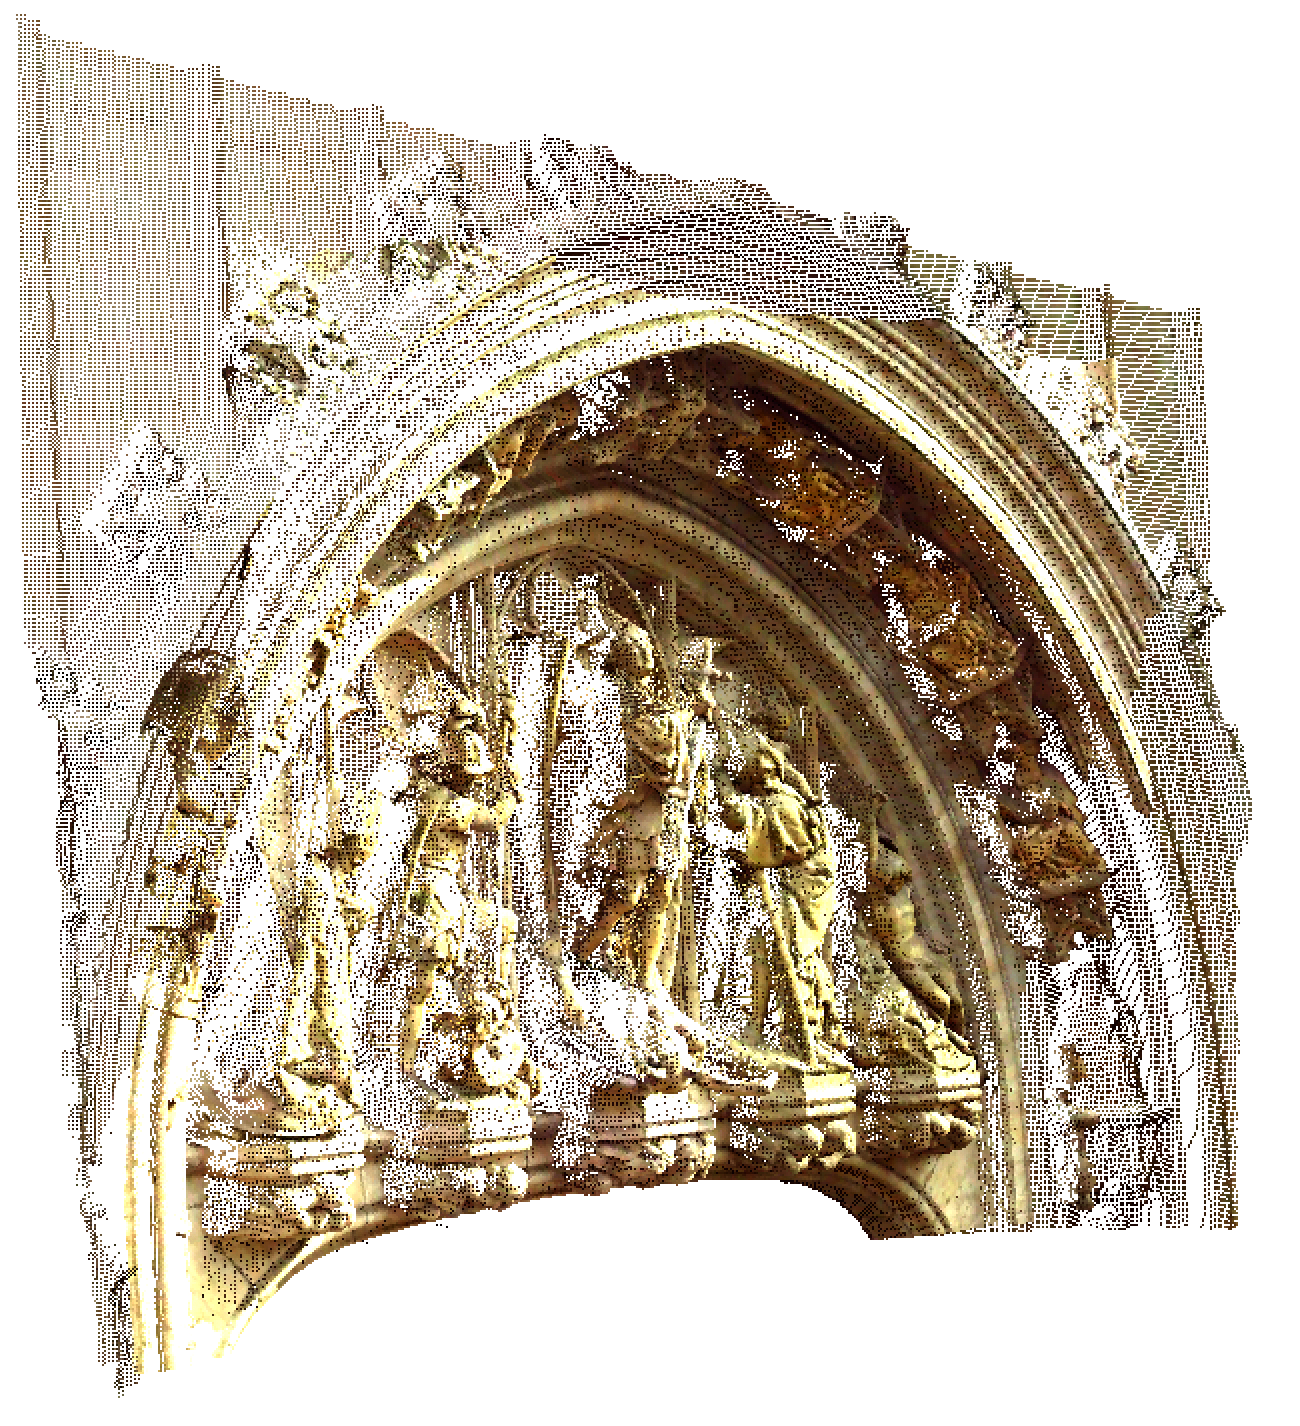
\includegraphics[width=.35\textwidth]{fig/ddp_icp_good.png}
\caption{Example of good registration of dessus-de-porte}
\label{fig:ddp_good}
\end{figure}
